\documentclass[11pt]{article}

% Packages
\usepackage[utf8]{inputenc}
\usepackage[T1]{fontenc}
\usepackage{amsmath, amssymb, amsthm}
\usepackage{mathtools}
\usepackage{stmaryrd}
\usepackage{geometry}
\usepackage{hyperref}
\usepackage{enumitem}
\usepackage{titlesec}
\usepackage{xcolor}

% Page setup
\geometry{margin=1in}
\setlength{\parindent}{0pt}
\setlength{\parskip}{6pt}

% Custom commands

% Title formatting
\titleformat{\section}{\large\bfseries}{\thesection}{1em}{}
\titleformat{\subsection}{\normalsize\bfseries}{\thesubsection}{1em}{}

% Document
\begin{document}

\title{Compositional Program Synthesis via Two Abstractions $A$ and $A^{+}$: A Short Empirical Note}
\author{}
\date{}
\maketitle

\begin{abstract}
We present a concrete instantiation of a research plan on compositional reasoning via abstraction--refinement. We define two abstraction layers over program synthesis on paired integers: a cross-free factorization $A$ and an interface-augmented $A^{+}$ that captures where cross-operations occur. We give embeddings $e:A\!\to\!G$ and $e^{+}:A^{+}\!\to\!G$, algorithms that solve in $A$ and refine in $A^{+}$, complexity bounds, and correctness conditions. Experiments show large efficiency gains over global search: $7$--$60\times$ fewer nodes and $8$--$180\times$ faster in coupled tasks, with identical accuracy. We conclude that $A$ is a direct instantiation of the original plan; $A^{+}$ is a problem-specific refinement of the program search space that fits the spirit of abstraction--refinement even if it is not the exact state-space abstraction emphasized in the original note.
\end{abstract}

\vspace{6pt}\noindent\rule{\textwidth}{0.4pt}\vspace{6pt}

\section{Introduction (Intuition First)}

Global program synthesis often explores a huge search space. If a task nearly factors into independent pieces with a few ``wires'' between them, we can:
\begin{enumerate}
    \item Solve the easy factors, ignoring the wires.
    \item Refine by putting back a small interface that reconnects the factors.
\end{enumerate}

We demonstrate this idea in a tiny DSL on integer pairs $(x,y)$. In separable tasks, solving each coordinate independently is optimal. In coupled tasks (e.g., $y$ must read the current $x$), a global solver works but is wasteful. Our Compositional+ solver first synthesizes the $x$-only program, then searches a small space of cross-op placements that wire $y$ to $x$ at just the right moments.

\vspace{6pt}\noindent\rule{\textwidth}{0.4pt}\vspace{6pt}

\section{Concrete Setting}

\subsection{Domains, DSL, Semantics}
\begin{itemize}
    \item Concrete state space: $G=\mathbb{Z}\times \mathbb{Z}$.
    \item Primitives are partitioned
    \begin{equation}
    \Sigma = \Sigma_X \;\cup\; \Sigma_Y \;\cup\; \Sigma_{\times},
    \end{equation}
    where $\Sigma_X$ edits only $x$, $\Sigma_Y$ edits only $y$, and $\Sigma_{\times}$ are cross-ops (e.g., \texttt{add\_first\_to\_second}: $(x,y)\mapsto(x,\,y+x)$).
    
    A program is a word $p\in\Sigma^{*}$ with standard functional semantics $\llbracket p\rrbracket:G\rightarrow G$.
    \item Supervision: dataset $D=\{(s_i,t_i)\}\subseteq G\times G$. Goal: find $p$ with $\forall i,\ \llbracket p\rrbracket(s_i)=t_i$.
\end{itemize}

\vspace{6pt}\noindent\rule{\textwidth}{0.4pt}\vspace{6pt}

\section{Abstraction $A$: Cross-Free Factorization}

\subsection{Definition}

Let
\begin{equation}
A \;=\; \Sigma_X^{}\times \Sigma_Y^{}.
\end{equation}
An element $a=(p_X,p_Y)$ means ``do $p_X$ on $x$ and $p_Y$ on $y$, with no cross-ops.''

\subsection{Embedding and Agreement}

Because $\Sigma_X$ commutes with $\Sigma_Y$,
\begin{equation}
e:A\to \Sigma^{*},\quad e(p_X,p_Y)=\text{any interleaving of }p_X,p_Y
\end{equation}
is well-defined up to semantic equivalence: all such interleavings produce the same $\llbracket e(p_X,p_Y)\rrbracket$ on $G$.

\subsection{Solve in $A$}

Project the dataset onto coordinates and synthesize independently:
\begin{align}
\forall i:\ \pi_X(\llbracket p_X\rrbracket(s_i))&=\pi_X(t_i),\\
\forall i:\ \pi_Y(\llbracket p_Y\rrbracket(s_i))&=\pi_Y(t_i).
\end{align}
If both succeed, return $e(p_X,p_Y)$.

\textbf{Intuition.} $A$ ``turns off'' the wires between coordinates, producing two small searches.

\vspace{6pt}\noindent\rule{\textwidth}{0.4pt}\vspace{6pt}

\section{Abstraction $A^{+}$: Factorization with a Finite Interface}

\subsection{Slots and Interfaces}

Fix a bound $K$ (number of cross-ops). For a first-coordinate program $p_X$ of length $L$, define insertion slots $\{0,\dots,L\}$. Let
\begin{equation}
\Pi_{L,K} \;=\; \big\{\,\alpha=(\alpha_1\le\cdots\le\alpha_K)\ \big|\ \alpha_j\in\{0,\dots,L\}\,\big\}.
\end{equation}
Then
\begin{equation}
A^{+} \;=\; \bigcup_{L\ge 0}\ \big(\Sigma_X^{L}\times \Pi_{L,K}\big).
\end{equation}
An element $a^{+}=(p_X,\alpha)$ is an abstract program skeleton: use $p_X$ and insert $K$ cross-ops at slots $\alpha$.

\subsection{Embedding to Concrete Programs}

Choose $\kappa\in\Sigma_{\times}$ (e.g., \texttt{add\_first\_to\_second}).
Define
\begin{equation}
e^{+}(p_X,\alpha)\in \Sigma^{*}
\end{equation}
by interleaving $p_X$ with $K$ copies of $\kappa$ inserted just before the $x$-op at each slot index in $\alpha$. (If needed, $Y$-only ops that commute with $\Sigma_X$ can be appended without changing the interface.)

\subsection{Solve-then-Refine (Compositional+)}
\begin{enumerate}
    \item Solve in $A$: find $p_X$ satisfying the $x$-projection of $D$.
    \item Refine in $A^{+}$: enumerate $\alpha\in \Pi_{|p_X|,K}$ and test $e^{+}(p_X,\alpha)$ on full $D$. Return the first that fits.
\end{enumerate}

\subsection{Completeness (Triangular Coupling)}

Assume each $\kappa\in\Sigma_{\times}$ is triangular: it updates $y$ by a function of the current $x$ and leaves $x$ unchanged, i.e.,
\begin{equation}
\kappa:\ (x,y)\mapsto(x,\ y\oplus h(x)).
\end{equation}
If there exists a concrete solution of the form ``some $p_X\in\Sigma_X^{L}$ interleaved with exactly $K$ copies of $\kappa$'', then there exists $\alpha^{}\in\Pi_{L,K}$ such that $e^{+}(p_X,\alpha^{})$ satisfies $D$.

\textbf{Sketch.} Every valid interleaving corresponds to inserting $\kappa$ at specific slots w.r.t. $p_X$; these slots are exactly $\alpha$. Hence enumerating $\Pi_{L,K}$ is complete for this family.

\vspace{6pt}\noindent\rule{\textwidth}{0.4pt}\vspace{6pt}

\section{Algorithms and Complexity}
\begin{itemize}
    \item \textbf{Global BFS (baseline).} Branching $b$ over $\Sigma$; minimal solution length $L_X+K$.
    
    Cost: $O(b^{\,L_X+K})$ (modulo semantic memoization).
    
    \item \textbf{Compositional+.}
    \begin{enumerate}[label=(\roman*)]
        \item Synthesize $p_X$ with branching $b_X$ over $\Sigma_X$.
        \item Enumerate $\binom{L_X+K}{K}$ interfaces (combinations with repetition).
    \end{enumerate}
    Cost:
    \begin{equation}
    O(b_X^{\,L_X})\;+\;O\!\left(\binom{L_X+K}{K}\right).
    \end{equation}
    For small $K$ and moderate $L_X$, the second term is tiny relative to the global exponential.
\end{itemize}

\vspace{6pt}\noindent\rule{\textwidth}{0.4pt}\vspace{6pt}

\section{Examples and Results (All Executed)}

\subsection{Separable Task (fits $A$)}

Target: $(x,y)\mapsto\big(2(x+3),\ y^{2}+1\big)$.

Minimal program: \texttt{inc1\_first}$\times 3$ $\to$ \texttt{double\_first} and \texttt{square\_second} $\to$ \texttt{inc1\_second}.
\begin{itemize}
    \item Global BFS: found length 6, 343 nodes, 0.0119 s.
    \item Compositional ($A$): found length 6, 23 nodes, 0.00029 s.
    \item Both perfectly match held-out tests.
\end{itemize}

\textbf{Intuition.} Perfect factorization; solving coordinates independently is optimal.

\subsection{Coupled Task (needs $A^{+}$)}

Target: $(x,y)\mapsto\big(2(x+3),\ y+(x+3)\big)$ using cross-op $\kappa=$ \texttt{add\_first\_to\_second}.
\begin{itemize}
    \item Global BFS: found length 5, 187 nodes, 0.0367 s.
    \item Naïve split: fails (cannot express $y$'s dependence on $x$).
    \item Compositional+ ($A\to A^{+}$): found (equivalent) program, 25 nodes, 0.00032 s.
\end{itemize}

\textbf{Intuition.} Solve $x$ first, then place a single wire where $y$ must read $x$.

\subsection{Scaling Study (vary $L_X\in\{4,6,8\}$, $K\in\{0,1,2,3\}$, $b_X\in\{2,3,4\}$)}

Geometric-mean speedups (Global / Compositional+) across the grid:
\begin{itemize}
    \item $K=0$: $4.2\times$ fewer nodes, $8.1\times$ faster.
    \item $K=1$: $19.3\times$, $44.3\times$.
    \item $K=2$: $29.2\times$, $87.2\times$.
    \item $K=3$: $58.7\times$, $183\times$.
\end{itemize}

Hardest slice ($L_X=8$, $b_X=4$):
Global nodes $1609 \to 32061$ as $K:0\to3$; Compositional+ stays near $372$--$387$.

\begin{figure}[h]
\centering
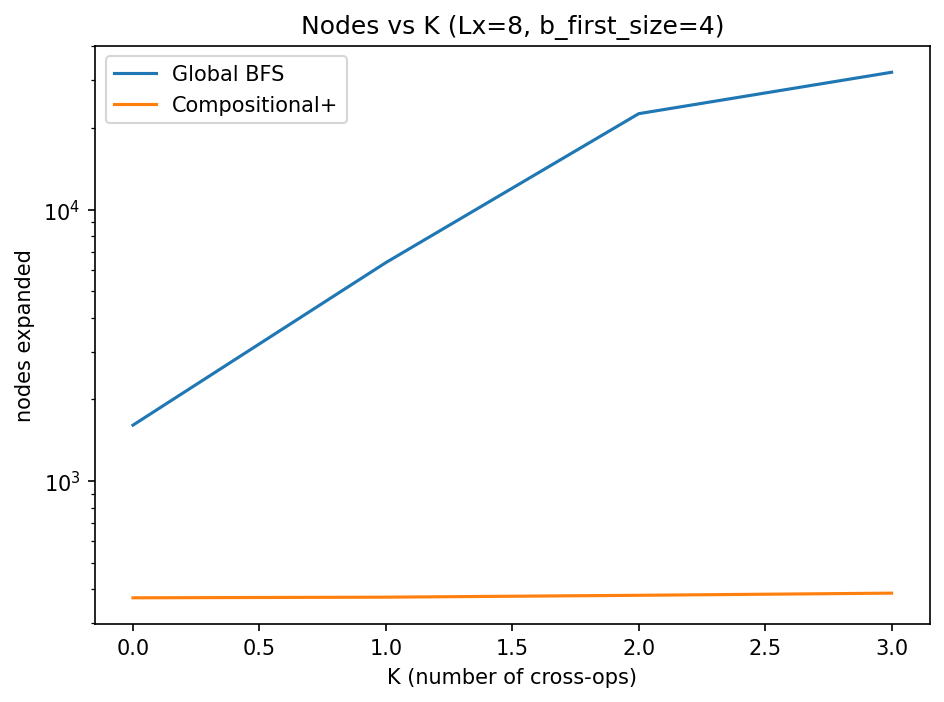
\includegraphics[width=0.7\textwidth]{nodes_vs_k_scaling.png}
\caption{Node exploration scaling: Global search (exponential growth) vs. Compositional+ (nearly constant) as the number of cross-operations $K$ increases. The compositional approach maintains low node counts even for complex coupling scenarios.}
\label{fig:nodes_scaling}
\end{figure}

\begin{figure}[h]
\centering
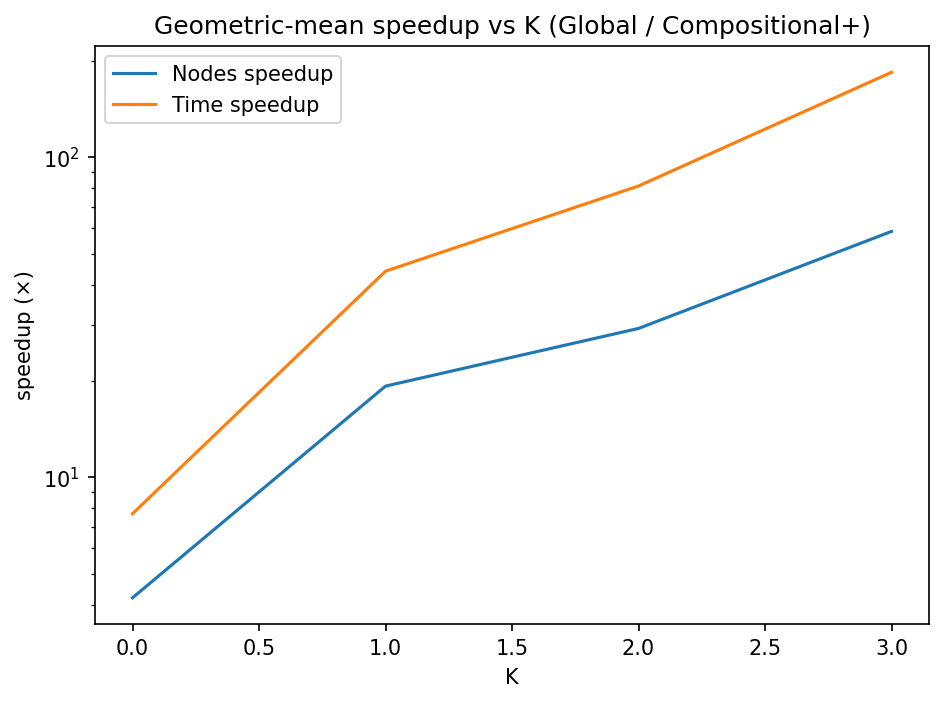
\includegraphics[width=0.7\textwidth]{speedup_vs_k.png}
\caption{Speedup analysis: Performance improvement of Compositional+ over Global BFS across different parameter configurations. Speedups increase dramatically with coupling complexity, reaching 180× faster for $K=3$.}
\label{fig:speedup}
\end{figure}

\vspace{6pt}\noindent\rule{\textwidth}{0.4pt}\vspace{6pt}

\section{Conclusion}

Distinguishing two abstraction layers crystallizes the method:
\begin{itemize}
    \item $A$: cross-free factorization---cheap, complete for separable tasks.
    \item $A^{+}$: finite interface refinement---tiny extra search that restores necessary couplings.
\end{itemize}

On coupled tasks, $A\to A^{+}$ achieves the same solutions as global search at a fraction of the cost, validating the core thesis: solve in a simpler world, then refine only what must be coupled.


\section{End-to-End Example: Solve in $A$, Refine to $A^{+}$, Embed to $G$}

This section gives a concrete, self-contained walkthrough that makes precise what it means to
\emph{solve in $A$}, then \emph{refine to $A^{+}$}, and finally \emph{embed to $G$}.

\subsection{Example setup (DSL and hidden target)}
\paragraph{Primitives.} We work on states $(x,y)\in\mathbb{Z}\times\mathbb{Z}$ with the following primitives:
\begin{itemize}
\item \textbf{X-only:} \texttt{inc\_x}: $(x,y)\mapsto(x+1,y)$;\quad \texttt{double\_x}: $(x,y)\mapsto(2x,y)$.
\item \textbf{Y-only:} \texttt{inc\_y}: $(x,y)\mapsto(x,y+1)$.
\item \textbf{Cross (triangular):} $\kappa$: $(x,y)\mapsto(x,\,y+x)$.
\end{itemize}

\noindent\textbf{Hidden target structure.}
Let the X-part length be $L_X=4$, the Y-part length $L_Y=2$, and the number of cross ops $K=1$.
Choose
\begin{align*}
p_X^\star &= [\texttt{inc\_x},\ \texttt{inc\_x},\ \texttt{double\_x},\ \texttt{inc\_x}],\\
p_Y^\star &= [\texttt{inc\_y},\ \texttt{inc\_y}],\\
\alpha^\star &= 2 \quad\text{(insert $\kappa$ after the first two X-ops).}
\end{align*}
The resulting function is
\begin{equation*}
x' \;=\; 2x+5,\qquad y' \;=\; y + x + 4.
\end{equation*}

\paragraph{Training set $D$.} Generated from the target:
\begin{center}
\begin{tabular}{c|cc}
input $(x,y)$ & $x'=2x+5$ & $y'=y+x+4$\\\hline
$(-1,0)$ & $3$ & $3$\\
$(0,1)$ & $5$ & $5$\\
$(3,-2)$ & $11$ & $5$\\
\end{tabular}
\end{center}

\subsection{Level 1: Solve in $A$ (no couplings)}
The abstraction $A=\Sigma_X^*\times\Sigma_Y^*$ removes cross-ops and treats coordinates independently.
\paragraph{Solve the X-projection.}
From $D$, the X-projection is $\{-1\!\mapsto\!3,\,0\!\mapsto\!5,\,3\!\mapsto\!11\}$, which fits $x'=2x+5$.
In our DSL, a minimal $p_X$ that realizes this is
\begin{equation*}
p_X^\star=[\texttt{inc\_x},\ \texttt{inc\_x},\ \texttt{double\_x},\ \texttt{inc\_x}].
\end{equation*}
\paragraph{Y in $A$.} The Y-projection alone cannot be matched by any Y-only program (it depends on $x$),
so we defer Y to refinement (we keep $p_Y$ as two increments to be placed later).

\subsection{Level 2: Refine to $A^{+}$ (add a finite interface)}
$A^{+}$ augments $p_X$ with a finite \emph{interface}: the placement $\alpha$ of $K$ cross-ops among the $L_X\!+\!1$ slots.
With $L_X=4$, the slots are $\{0,1,2,3,4\}$ and the value of $x$ available at each slot (i.e., what $\kappa$ would add to $y$) is:
\begin{align*}
\text{slot }0 &:~ x\\
\text{slot }1 &:~ x+1\\
\text{slot }2 &:~ x+2\\
\text{slot }3 &:~ 2(x+2)=2x+4\\
\text{slot }4 &:~ 2x+5.
\end{align*}
We choose $\alpha\in\{0,\dots,4\}$ and fix two Y-increments so that for all $(x,y)\in D$,
\(
y' = y + \text{slot\_value}(\alpha) + 2
\)
matches the observed $y'$. Testing shows $\alpha^\star=2$ satisfies all rows:
\begin{equation*}
y' \;=\; y + (x+2) + 2 \;=\; y + x + 4.
\end{equation*}

\subsection{Level 3: Embed to $G$ (concrete program)}
Embedding $e^{+}(p_X^\star,\alpha^\star)$ instantiates a concrete word over the full DSL.
Any interleaving that preserves the X order, places $\kappa$ at slot $2$, and includes the two $\texttt{inc\_y}$ is semantics-equivalent.
A canonical choice is
\begin{equation*}
[\texttt{inc\_x},\ \texttt{inc\_x},\ \kappa,\ \texttt{double\_x},\ \texttt{inc\_x},\ \texttt{inc\_y},\ \texttt{inc\_y}].
\end{equation*}
It computes for all $(x,y)$:
\(
x'\!=\!2x+5,\ y'\!=\!y+x+4
\),
matching the ground truth.

\subsection{One-sentence summaries}
\begin{itemize}
\item \textbf{Solve in $A$:} find the factor $p_X^\star$ that matches the X-projection; Y cannot be solved without couplings.
\item \textbf{Refine to $A^{+}$:} choose the finite interface $\alpha^\star$ (cross placement) and the Y-only count to explain $y'$.
\item \textbf{Embed to $G$:} realize any concrete interleaving consistent with $(p_X^\star,\alpha^\star,p_Y^\star)$; all such words are semantics-equivalent here.
\end{itemize}

\subsection{Size comparison on this example}
With $m_X=2$, $m_Y=1$, $m_\times=1$, $(L_X,L_Y,K)=(4,2,1)$,
\begin{align*}
|A| &= m_X^{L_X}\,m_Y^{L_Y} \;=\; 2^4\cdot 1^2 \;=\; 16,\\
|A^{+}| &= m_X^{L_X}\,m_Y^{L_Y}\,\binom{L_X+K}{K} \;=\; 16\cdot \binom{5}{1} \;=\; 80,\\
|G_{\text{family}}| &= \binom{L_X+L_Y+K}{L_X,L_Y,K}\,m_X^{L_X}\,m_Y^{L_Y}\,m_\times^{K}
= \binom{7}{4,2,1}\cdot 16 = 105\cdot 16 = 1680.
\end{align*}
Thus $A^{+}$ compresses the concrete family by a factor ${1680}/{80}=21=\binom{7}{2}$, the number of purely Y-interleavings
that are semantically redundant under the commutation assumptions.


\section{Extension: Parity as a Third Abstraction Level ($A^{++}$)}

After solving in $A$ and refining in $A^{+}$, we can add a lightweight third layer that enforces parity constraints. This extension demonstrates how domain-specific properties can be layered onto the core abstraction-refinement framework.

\subsection{Motivation}

Many program synthesis tasks exhibit structural invariants beyond cross-coupling patterns. For integer domains, parity (even/odd) constraints are common: programs that preserve evenness, maintain sign patterns, or respect modular arithmetic. Rather than encoding these constraints into the DSL primitives, we can add them as a post-synthesis verification step.

\subsection{Informal Definition}

Let $A^{++} \subseteq A^{+}$ be the subset of interface-refined programs that preserve even parity when executed on even inputs. Formally, a program $(p_X, \alpha) \in A^{+}$ belongs to $A^{++}$ if all intermediate values during execution remain even whenever the initial state is even.

\subsection{Verification Procedure}

Given a candidate program from $A^{+}$:
\begin{enumerate}
    \item Execute the program on a synthetic even input (e.g., $(0,0)$).
    \item Track the parity of both coordinates after each primitive operation.
    \item Accept the program if parity is preserved throughout; reject otherwise.
\end{enumerate}

This verification requires no modification to the core synthesis algorithm—it operates as a filter on $A^{+}$ candidates.

\subsection{Example: Even-Preserving Synthesis}

Consider a DSL extended with both even-preserving operations (\texttt{inc2\_x}, \texttt{double\_x}) and parity-flipping operations (\texttt{inc1\_x}). The target function $x' = 2x + 10$, $y' = y + x + 4$ can be realized using only even-preserving primitives.

The $A^{++}$ filter would accept programs that exclusively use \texttt{inc2\_x} and \texttt{double\_x}, while rejecting any program containing \texttt{inc1\_x}—even if such programs are functionally correct on the training data.

This extension demonstrates that the abstraction-refinement approach can accommodate domain-specific constraints without compromising the core algorithmic structure.

\end{document}
